%
A bolometer for \bbonu-decay searches consists of a dielectric crystal, which contains the isotope of interest, coupled to a temperature sensor. When the bolometer is cooled to very low temperatures ($<20$~mK for crystals with masses in the 0.1--1~kg range), the energy deposited in the crystal by interacting particles can be measured with high precision as a rise in temperature. This technique, originally proposed for rare-event searches in the early 1980s \cite{Fiorini:1983yj}, can provide an energy resolution at the few per-mil level (FWHM) at 3~MeV and a total efficiency at the 70\%--90\% level. Bolometer-based detectors ---\thinspace at very different scales and maturity levels \thinspace--- have been used to search for \bbonu\ in six different nuclides ($^{48}$Ca, $^{82}$Se, $^{100}$Mo, $^{116}$Cd, $^{124}$Sn and $^{130}$Te) since the 1990s.

The MiDBD experiment \cite{Arnaboldi:2002te} at LNGS was the first bolometric array with large-mass crystals. It consisted of 20 TeO$_2$ bolometers of 340~g each ($3\times3\times6$~cm$^3$ crystals). MiDBD proved that an energy resolution of 5~keV at the $Q$ value was within reach, and achieved a background rate of less than 1~\ckky\ in the region of interest around \Qbb. With a total exposure of 4.25~kg~yr, MiDBD set the limit $T_{1/2}^{0\nu}(\Te{130}) > 2.1\times10^{23}$~years at 90\% CL. 

CUORICINO \cite{Andreotti:2010vj}, an array of 62 TeO$_2$ crystals, improved on the MiDBD results after running between 2003 and 2008 at LNGS, accumulating a total exposure of 19.75~kg~yr. It set a lower bound on the \Te{130} half-life of $2.8\times10^{24}$~years at 90\% CL. 

The latest step in this long series of TeO$_2$ bolometric detectors is CUORE \cite{CUORE:2021mvw}, currently taking data at LNGS and consisting of 988 bolometers with a mass of about 750~g each, corresponding to about 200 kg of \Te{130}. So far, the experiment has set a lower limit of $2.2\times10^{25}$~years on the half-life of \Te{130} for an exposure of 288.8~kg~yr. The background rate, $(1.49\pm0.04)\times 10^{-2}$~\ckky, is dominated by energy-degraded $\alpha$ particles generated by surface contamination. CUORE will continue to take data until it reaches its design \Te{130} exposure of 1~ton~yr. 

Scintillating bolometers could bring an additional handle for the discrimination between signal and background \cite{Pirro:2005ar}. In these devices, the crystal containing the isotope of interest is a scintillator, and a second auxiliary bolometer is operated close to it to register the emitted scintillation light. The simultaneous detection of heat and scintillation allows one to distinguish $\alpha$ particles from electrons or $\gamma$ rays thanks to their different light yield and signal shape, eliminating the dominant background source observed in CUORE. This and other background reduction techniques are the subject of an intense, world-wide R\&D program; for more details, see, for example, \cite{Zolotarova:2021inw} and references therein.

%%%%%
\begin{figure}[t!b!]
\begin{center}
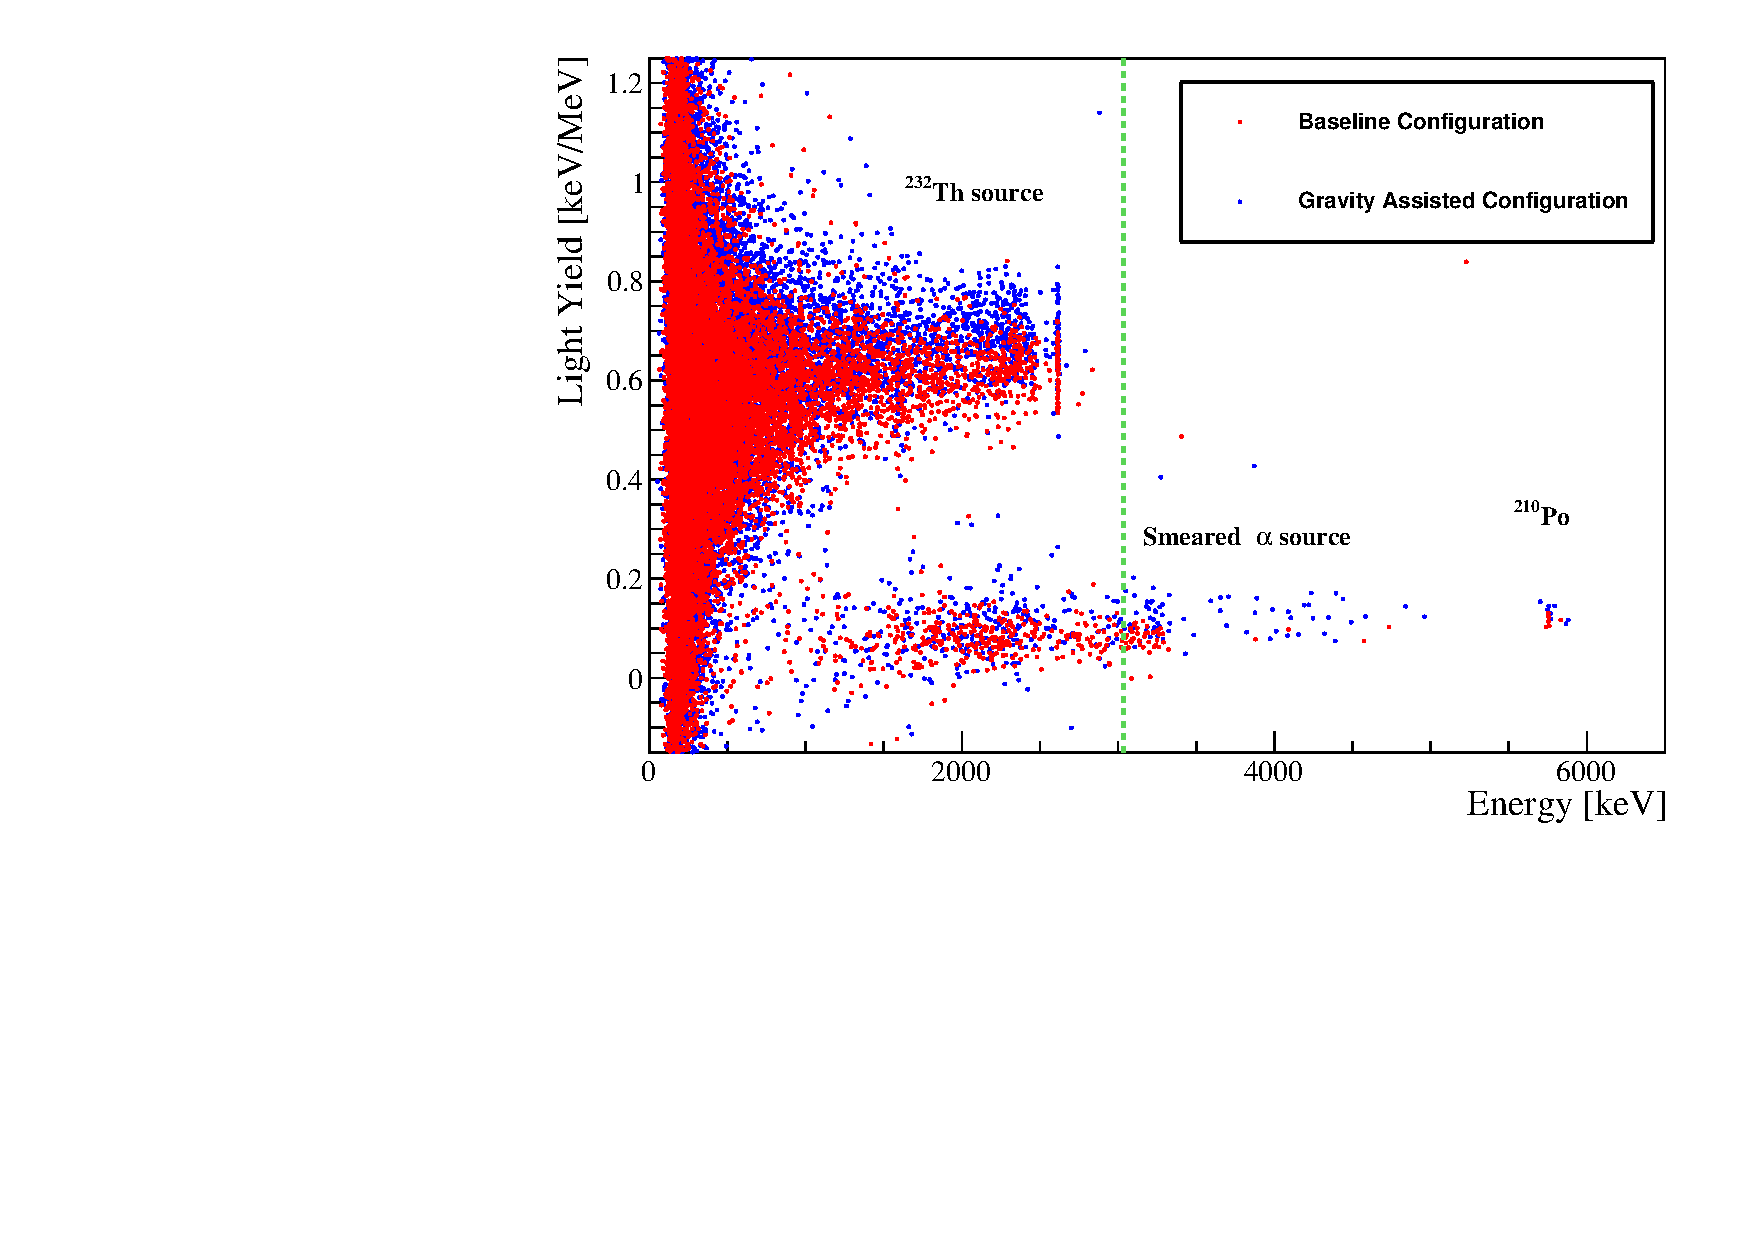
\includegraphics[width=0.8\textwidth]{img/cupid.pdf}
\end{center}
\caption{Light yield per unit energy as a function of the energy deposited in the LMO crystal, for two different configurations under study as part of the CUPID detector optimization process. The green vertical line indicates the Q-value of \Mo{100}. Taken from \cite{CUPID:2022opf}.} \label{fig:cupid}
\end{figure}
%%%%%

The CUPID (CUORE Upgrade with Particle IDentification) \cite{CUPID:2019imh} project aims to improve the half-life sensitivity of CUORE by 2 orders of magnitude increasing the source mass and reducing the background by using scintillating bolometers based on lithium molybdate (Li$_2$MoO$_4$, or LMO) crystals highly enriched in \Mo{100}. The particle identification performance of the first CUPID detector module, exploiting the light-to-heat ratio, is shown in Fig.~\ref{fig:cupid}. CUPID-Mo \cite{Augier:2022znx}, a demonstrator experiment consisting of an array of 20 Li$_2$MoO$_4$ enriched in \Mo{100} to about 97\%, was installed at the Laboratoire Souterrain de Modane (LSM), France, and collected a total exposure of 1.48~kg~yr between 2019 and 2020. The scintillation light signal allowed a complete rejection of $\alpha$ particles, while an energy resolution of $7.7\pm0.4$~keV (FWHM) was measured at 3034~keV. This performance lead to a lower limit on the \bbonu\ half-life of \Mo{100} of $1.8\times10^{24}$~years at 90\% CL. 

The AMoRE \cite{Kim:2022uce} (Advanced Mo-based Rare process Experiment) project is also searching for the \bbonu\ of \Mo{100}, but using scintillating bolometers of \Mo{100}-enriched and \Ca{48}-depleted calcium molybdate crystals. Tests have demonstrated that CaMoO$_4$ crystals produce the brightest scintillation light among all of the molybdate crystals, both at room and at cryogenic temperatures. The AMORE-pilot experiment, carried out between 2016 and 2018 utilizing six crystals with a total mass of 1.9~kg, achieved a half-life sensitivity of $3.43\times10^{23}$~yr at 90\% CL and demonstrated the fundamentals of the technology. The current phase of the experiment, AMoRE-I, has been running at the Yangyang Underground Laboratory (Y2L) with a 6.2~kg array of thirteen Ca$^{100}$MoO$_4$ and five Li$_2$$^{100}$MoO$_4$ crystals and aims at a background level of the order of 0.01~counts~keV$^{-1}$~kg$^{-1}$~year$^{-1}$ and a half-life sensitivity of $10^{24}$ years. The next phase of the experiment, AMoRE-II, will make use of a total mass of approximately 100 kg of \Mo{100}.
